% ========== Chapter 4
 
\chapter {\uppercase{Evolution of gene regulatory networks in prokaryotes}}
\label{chap:4}

The evolutionary success of an organism is a testament to its inherent capacity to keep pace with environmental conditions that change over short and long periods. Mechanisms underlying adaptive processes are being investigated with renewed interest and excitement. This revival is partly fueled by powerful technologies that can probe molecular phenomena at a systems scale. Such studies provide spectacular insight into the mechanisms of adaptation, including rewiring of regulatory networks via natural selection of horizontal gene transfers, gene duplication, deletion, readjustment of kinetic parameters, and myriad other genetic reorganizational events. In this chapter, I discuss advances in our understanding of principles that shape evolution of gene regulatory networks (GRNs) for dynamic adaptation to environmental change. \\

\noindent This chapter has been adapted from: \\

\noindent Brooks AN, Turkarslan S, Beer KD, Lo FY, Baliga NS. Adaptation of cells to new environments. (2011) \emph{Wiley Interdiscip Rev Syst Biol Med}. 3(5): 544–561\\

\paragraph{Chapter Highlights}

\begin{itemize}
\item Microbes have adapted to diverse environmental conditions 
\item Mechanism of adaptation depends on how fast and frequently the environment changes
\item GRN evolution contributes to environmental adaptation in microbes
\item Evolutionary processes in microbes can be studied in the lab 
\end{itemize}

\section{Summary}

GRNs can be rewired through several genetic reorganizational mechanisms, including gene duplication, deletion, mutation, and horizontal transfer. Temporal properties of environmental variability influences what types of molecular changes are permitted and/or preferred. Some microbes may have evolved an ability to anticipate coupled environmental changes. 

\section{Introduction}

Microorganisms experience myriad environmental factors over their evolutionary history, including those that remain essentially constant over long periods (e.g. geological epochs), change slowly (e.g. general increase in annual temperatures), fluctuate periodically (e.g. day-night cycles and seasonal variations), or change frequently and somewhat randomly (e.g. unpredictable nutrient loading).  These changes occur over diverse timescales, ranging from the lifetime of an individual cell to multiple generations. Accordingly, microbes have evolved unique strategies to deal with the peculiarities of their environment \cite{galhardo_mutation_2007}.  Characteristic examples include adaptation to extreme environmental niches \cite{kennedy_understanding_2001,kushner_microbial_1978}, entrainment of phototrophs to day-night cycles \cite{woelfle_adaptive_2004,ouyang_resonating_1998}, and the physiological adjustment of \eco as it passes through the human intestine \cite{mitchell_adaptive_2009}.  Organisms respond to short term environmental changes by reversibly adjusting their physiology to maximize resource utilization while maintaining structural and genetic integrity by repairing and minimizing damage to cellular infrastructure \cite{huisman_sensing_1994,ram_community_2005} thereby balancing innovation with robustness. Naturally, physiological response networks emerge as products of evolution by natural selection where they can lend reproductive or fitness advantage, particularly when the environmental change is recurrent \cite{hochachka_biochemical_2002}.

Environmental adaptation of biological systems can be considered from three evolutionary perspectives: (i) acclimation of existing cellular machinery to operate optimally in a new environmental niche; (ii) acquisition of entirely new capabilities through horizontal gene transfer or neofunctionalization of gene duplications and (iii) reorganization of network dynamics to appropriately adjust existing physiological processes to match dynamic environmental changes. The first type of adaptation can arise through two types of events that differ dramatically in duration. Simple mutations can greatly increase fitness over very short time frames (within one or few generations). Prominent examples of short-term adaptive events include resistance to drugs \cite{schrag_adaptation_1997,spain_adaptation_1983} and altered nutrient conditions \cite{finkel_evolution_1999}. Alternatively, complex mutations in multiple loci may accumulate over very long time frames, such as the evolution of acidic protein surfaces in halophilic archaea \cite{kennedy_understanding_2001,gribaldo_origin_2006,soppa_genomics_2008}.  While the initial transfer of adaptive genes by HGT occurs rapidly \cite{babic_direct_2008}, full integration of laterally transferred component(s) typically occurs over longer time frames (10s of millions of years), where HGT events often require regulatory rewiring to function optimally in the context of existing cellular networks \cite{lercher_integration_2008}.  Finally, physiological readjustment occurs both because of genetic and physiological robustness to withstand stress that accumulates over many generations and latent genetic variance that is revealed after environmental perturbation \cite{rutherford_genotype_2000}. 

Here, we focus on the evolution of adaptive mechanisms for acclimation to recurrent yet transient environmental changes.  When transient changes are recurrent they select for genetic traits that confer fitness by improving the ability of an organism to rapidly and reversibly adjust physiology to match current environmental conditions. These traits manifest at varying hierarchies of genetic information processing, from receptors for sensing environmental factors, to signal relay, transcriptional, post-transcriptional, translational and post-translational control mechanisms, and also at the metabolic level through modulation of enzyme function (affinities, kinetics etc.).  Such adaptive changes occur over intermediate time frames (upwards of 100s of generations in \eco; \cite{tagkopoulos_predictive_2008}) and, surprisingly, they arise repeatedly and in some cases with some regularity in distinct lineages \cite{chaffron_global_2010} Fitness, or the number of surviving offspring after one generation \cite{barton_evolution_2007}, is a complex property that emerges from the integration of changes at all these levels. A holistic systems approach, therefore, is necessary to fully appreciate how these varied mechanisms work together when an organism adapts to a new environment.  

For the purpose of our discussion, we define environmental conditions to include both abiotic physical variables (such as light and temperature) and biotic components (such as other co-inhabiting organisms).  Additionally, we restrict our analysis to asexual prokaryotic systems (including both bacteria and archaea) in which the dynamics and mechanisms of genetic evolution lack the pervasive variation that recombination by sexual reproduction promotes. Sexual populations also may not experience signatures of selection prevalent in asexual populations, such as ‘classic’ sweeps associated with unconditionally advantageous mutations \cite{burke_genome-wide_2010}. The reader should note, however, that the physiology of archaea and bacteria diverge substantially, with archaea sharing startling similarity to eukaryotes. Infrequently, we may explicitly refer to findings in eukaryotes that reflect mechanisms that likely also occur in prokaryotic systems. 

This chapter will bridge the conceptual gap between adaptation, which by definition requires heritable genetic change \cite{barton_evolution_2007}, and physiological readjustment, which is a product of adaptation that equips organisms to attune their physiology to dynamic changes in their environments. We will suggest how systems-level methodologies and insights can be applied to better understand the strategies living systems employ to withstand and in some cases take advantage of change in their environments. 

The fields of microbiology, molecular evolution, and systems biology are expansive – it would be impossible to cover all adaptive mechanisms and scenarios that may influence the evolution of natural microbial populations. Instead, we will highlight major themes and new insights in microbial evolution while demonstrating how the principles of systems biology can be leveraged to develop a more comprehensive, integrative understanding of cellular adaptation to new environments. Throughout our analysis we will point the reader to other outstanding reviews that complement our discussion.
  
\section{Types of adaptations and associated mechanisms} 

\subsection{What is adaptation?}   

When we say that an organism has adapted to its habitat, we imply that it has evolved molecular mechanisms that allow it to grow optimally under the spatiotemporally varying physicochemical conditions of its environment. Evolution, however, is an unfinished process. Organisms chase fitness optima in constantly changing environments. Subtle fitness differences between individuals (due to genomic plasticity or metabolic flexibility) and phylogenetic complexity (i.e. numbers and diversity of species within a community) can lead to the diversification of species or the extinction of less fit genotypes over time \cite{kassen_toward_2009}. Although many adaptive mutations are lost by random chance (as a result of genetic drift), mutations that confer significant selective advantage have a greater propensity to become fixed within the population, especially in large populations \cite{orr_theories_2005}.  If selection imposed by the environment is particularly strong, fitness-enhancing genotypes will rapidly rise in frequency in the population, often carrying associated, possibly detrimental, genes along with them  (i.e. selective sweep) \cite{papadopoulos_genomic_1999} and interfering with one another via clonal interference \cite{de_visser_clonal_2006}. 

\subsection{Adaptation to linked environmental changes: general stress response or anticipatory behavior?}   

Conditions within natural environments can change continually over long periods, periodically, or transiently and unpredictably.  In the context of evolution, these environmental changes occur simultaneously albeit on different timescales and exert selective pressure to enrich genotypes well matched to particular ecosystems.  Not surprisingly, the repertoire of analogous solutions that characterizes success in a given environment can be similar across diverse organisms occupying similar habitats, suggesting convergent evolution of adaptive solutions that were discovered independently in divergent lineages \cite{lauro_unique_2007,hentschel_molecular_2002}.  While a significant fraction of these responses are condition-specific, most organisms have also evolved robust generalized mechanisms to deal with shared aspects of stress resulting from diverse kinds of environmental changes.  In yeast, for example, a set of ~900 genes responds similarly to a diverse array of environmental stresses, sharing common regulatory themes mediated by Yap1p, Msn2p, and Msn4p \cite{gasch_genomic_2000}. This generalized stress response typically includes activation of heat shock proteins, phage shock proteins, and oxidative stress response proteins \cite{causton_remodeling_2001,he_positive_2010}, although there are notable examples in \textit{Candida albicans} and \halo where the central role of general stress response has been called into question \cite{enjalbert_stress-induced_2003,kaur_coordination_2010}.  The alternate perspective offered by these studies is that changes in environmental variables are physically linked and do not occur in isolation. Elevated temperatures, for example, induce a number of associated changes in environmental conditions, including decrease in oxygen solubility \cite{whitehead_diurnally_2009}. Theoretical and experimental work in diverse species suggests that organisms can learn to take advantage of this natural co-variation between environmental parameters (e.g. temperature and oxygen), thereby displaying `anticipatory behavior' \cite{tagkopoulos_predictive_2008,whitehead_diurnally_2009,wolf_memory_2008}.  B. subtilis, for example, retains short-term and long-term memories to inform sporulation dynamics and degradative enzyme synthesis \cite{wolf_memory_2008}.

Coupled environmental variables have important evolutionary implications that can be assessed by assaying the fitness consequences upon artificially decoupling such associations in the lab.  Relative to laboratory populations evolved in an inverted environment, wild-type \eco has a fitness disadvantage when naturally linked parameters, such as temperature and oxygen, are decoupled artificially. Likewise, cyanobacteria mutants with non-functional circadian clocks are less fit and out-competed by their wild-type counterparts \cite{johnson_cyanobacterial_2008}.  The enhanced fitness conferred by diurnal entrainment can be attributed to anticipation of predictable, associated stresses such as damaging UV radiation \cite{woelfle_adaptive_2004}.   Adaptation to stress may also prepare cells to better respond to future stresses. \textit{Vibrio parahaemolyticus}, for example, has a greater tolerance to acidity and temperature stresses following growth in media containing 3\% NaCl versus 1\% NaCl concentrations \cite{whitaker_modulation_2010}.  On the other hand, adaptation to a subset of environmental factors could come at a cost of sacrificing tolerance to others. Propionate adaptation of \textit{Salmonella enteritidis}, for instance, leads to enhanced resistance to stresses experienced inside the host but overall decrease in infectivity \cite{calhoun_effect_2010}.  For all these reasons, we need to appreciate the high degree of connectedness within environmental networks to interpret causes and functional consequences of complex biological responses.   

\section{Role of the environment in shaping GRN evolution: time matters} 

\subsection{Long-term adaptation}   

Some environmental conditions seldom change. We define long-term adaptation as the response to environmental conditions that remain relatively constant throughout the lifetime of a species. For organisms, this represents the most fundamental level of adaptation. Over many thousands to millions of years or longer, the internal architecture of the cell changes to accurately match the general features of the habitat it occupies. Typically, the features that reflect long-term environmental adaptation are deeply ingrained in the structure of the genome, regulatory schemas, or even the molecules of the cell themselves. These molecular artifacts reflect the organism's uphill struggle towards increased fitness in an environment that changes (being directly modified by biotic factors and even the organism itself) yet remains mostly constant over long timescales. Complete reversion of these features would be difficult, if not impossible, for an organism to achieve over short time scales, suggesting that cells are poorly adapted to large variations in these environmental parameters. \halo, for example, thrives in high salt conditions. While \halo can withstand lower salt concentrations (as low as 2.5M), anything below this concentration is lethal to cells. Adaptation to high salt conditions requires a number of significant structural changes in the cell, including global alterations at the level of DNA, RNA and protein composition \cite{dassarma_post-genomics_2006}. In high salt, water activity is low; this has profound consequences for enzymatic activity and the structural integrity of the cell membrane and genome. Adaptation to high-salt conditions has required the evolution of a highly-acidic proteome, high genomic GC content, and increased intracellular concentration of potassium cation \cite{oren_microbial_2008}.  Other factors including gene redundancy have been reported to enhance survival in fluctuating salt conditions. \textit{Salinibacter ruber}, for instance, possesses two or more copies of several essential genes. It has been proposed that slight differences in the amino acid composition of two versions of the same protein (ecoparalogs) might allow \textit{Salinibacter} to survive broader fluctuations in salt concentration \cite{sanchez-perez_adapting_2008}.  These strategies for thriving in hypersaline environments are generally utilized by diverse halophillic archaea.  Halophilic bacteria and eukaryotes, on the other hand, have independently evolved alternate mechanisms such as overproduction of organic osmolytes (sugar and amino acid-derivatives) to live in high salt environments \cite{oren_microbial_2008}.
 
Adaptation to temperature is another well-studied example of molecular response to long-term environmental pressures. While all microbial species are adapted to some range of permissive temperatures, interesting mechanistic examples of thermal adaption have been reported in both extreme warm and cold environments. Psychrophillic organisms occupy extremely cold ecosystems (permanent temperatures below 5C) located deep in the ocean, and in polar and alpine regions. The habitats colonized by psychrophiles are of particular interest because they constitute more than three-quarters of the Earth's surface \cite{feller_psychrophilic_2003}. Similarly, hyperthermophiles (optimal growth temperature $>$80C) occupy high temperature habitats. These organisms are so well adapted to their environments that, under some conditions, their doubling times approach that of \eco grown at 37C \cite{feller_psychrophilic_2003}. In both cases, the microorganisms that occupy these habitats have evolved enzymes and metabolic strategies that allow them to survive and proliferate at temperatures that would be restrictive or lethal to mesophilic organisms. To withstand these extreme temperatures, microbial species have evolved molecular mechanisms that regulate membrane fluidity and conformational flexibility of proteins, and produce thermo-stable protein variants, all of which are significantly challenged at extreme temperatures \cite{feller_life_2007,vieille_bivalent_2001}. While the specific mechanisms employed to combat extreme temperatures vary across species, common mechanisms, such as increased protein stability through ion pairs, hydrogen bonding, hydrophobic interactions, disulfide bridges, packing, and intersubunit interactions at high temperatures and increased protein flexibility and membrane fluidity and exopolysaccharide production at low temperatures, are common aspects of cellular adaption to extreme environments \cite{jaenicke_protein_1991}. Like the halophilic organisms described earlier, thermophiles and psychrophiles occupy environments that impose a number of additional harsh constraints on living systems (including metal ion concentrations, nutrient limitation, and sometimes increased pressure), making them useful models to understand adaptation to stressful conditions. 

\subsection{Short-term adaptation} 

Environmental variables can fluctuate in unanticipated ways. Such variations are often stressful and, depending on severity, might drive selection of genotypes that are better suited to readjust physiology to manage and mitigate the consequences of stress. Genotypes can be selected on the basis of either genetic or non-genetic components. Asymmetric cell division, in which mother and daughter cells receive disproportionate numbers of molecules, alters the dynamic behavior of cells in response to environmental change and may lead to the selection of genotypes that do not necessarily contain heritable allelic alterations, but rather exhibit a temporary, dynamic state compatible with the altered environment. Sporulation in \textit{B. subtilis}, for instance, couples asymmetric morphological changes with differential gene expression between the forespore and mother cell (Reviewed in \cite{barak_where_2005}), leading to divergent cell fate. Due to asymmetric cell division, daughter cells may receive more or fewer ribosomes, transcription factors, or other cellular components, each of which might  contribute to their success (or failure) in new environments. Phase variation (or phenotype switching) is another mechanism (non-genetic, though heritable alteration) by which microbial populations leverage stochastic variations in cell components to respond to uncertainty in environmental fluctuations \cite{veening_bistability_2008}. Genetic alterations, on the other hand, can occur anywhere within the cellular hierarchy; advantageous mutations may be located within proteins, affecting the stability or kinetic parameters of the protein, or within regulatory sequences, affecting when, where, and how much of a biological product is made. A common feature of these alterations, however, is that they tend to be simple, i.e. they are the product of one or a few adaptive mutations that spontaneously occur in response to the new environment or preexisting neutral or buffered mutations whose consequence is revealed by perturbation.In this sense, these adaptations are flexible, being easily gained and subsequently lost by genetic drift. The inherent plasticity of these mutations makes them especially important for physiological adaptation, as slight changes can drastically alter the dynamic response of an organism to stress. Short-term adaptation is tightly coupled to the longer-term adaptive mechanisms previously described. Temporary changes in long-term environmental trends may elicit genetic alterations that are short-lived, only becoming fixed within the population and canalized into regulatory programs if the stress that has elicited the advantageous mutation surpasses a temporal threshold, becoming a regular feature of the environment. Numerous studies have investigated mechanisms of adaptation to altered growth temperature \cite{bennett_rapid_1990,bennett_experimental_2007}, nutrient composition \cite{cooper_experimental_2010,blount_historical_2008} and population structure \cite{zinser_escherichia_2004}.  Universally, these studies find that fitness to a new environment increases rapidly over the first several thousand generations \cite{lenski_dynamics_1994,barrick_genome_2009}.  Surprisingly, adaptive mutations discovered in the lab typically occur in one or a few genes, reflecting the earliest events in the adaptive process. Only four mutations in \eco, for example, are responsible for gaining growth advantage in stationary phase: one in the stationary-phase sigma factor , one in the leucine-responsive regulatory protein, two genomic rearrangements of IS5 transposon insertion sequences, and a mutation in the \textit{sgaC} gene \cite{zinser_escherichia_2004}.

Short-term, stressful environmental perturbations may also specifically induce increased rates of mutation, potentially facilitating adaptive evolution by rapid exploration of a broader genotypic space. In response to nutrient starvation, for example, the DNA damage and cell-cycle checkpoint control response (SOS response pathway) is induced in \eco. Following induction of this pathway, cells experience higher rates of mutation due to inhibition of mismatch repair and recombinational break repair, and induction of a mutator DNA polymerase \cite{rosenberg_evolving_2001}. In addition, some genetic loci exhibit a disproportionatly high frequency of mutation during hypermutation. These mutational ‘hot’ spots may reflect regions of the genome that are more readily modified and thereby adaptive. Taken together, these observations suggest that organisms might possess the capacity to introduce a bias in the distribution of mutational variation along its chromosome(s).  

\section{Adaptation through rewiring GRNs} 

Systems-level coordination of cellular functions is accomplished by gene regulatory networks (GRNs) \cite{mcadams_evolution_2004}  The general form and features of biological networks are illustrated in Figure \ref{fig:chap4:networks}. Central to all GRNs is the interaction of TFs and their cognate DNA binding sites.  Remarkably, the origin of DNA-binding domains (DBDs) in all present day TFs can be traced to a few ancestral classes, such as winged-helix and zinc ribbon domains \cite{babu_structure_2004}.  This raises important questions regarding the evolutionary process(es) that led to the diversification of these few DBDs to create a vast array of distinct DNA binding specificities.  It could be argued that the common origins of DBDs within TFs and their division into related classes (protein families) should help characterize GRNs in one organism and suggest projections of that information onto orthologous systems in phylogenetically related species.  Functions of even structurally similar transcription factors (TFs), however, can diverge substantially through alterations in regulatory domains of either the transcription factor itself or the cis-regulatory sequences of downstream target genes. The divergence of DNA binding specificities and allosteric domains of two FNR (fumarate and nitrate reduction) family TFs in E. coli and B. subtilis are case in point.  As result of subtle DNA binding differences, FNR in E. coli controls 135 genes whereas its counterpart in B. subtilis regulates only 8 genes \cite{lozada-chavez_role_2008}.  Importantly, this result demonstrates that species-specific coevolution of interacting partners (in this case FNR and the target promoters) prohibits simple projection of TF-binding orthologies across species, even when the genes involved share recent ancestry.  On the other hand, this finding underscores the flexibility of GRNs – malleability of regulatory network topology can promote variation in gene expression that acclimates a species to the nuances of its environment \cite{lopez-maury_tuning_2008}.

Gene regulatory networks evolve through a number of molecular mechanisms that vary in frequency and magnitude of effect. Figure \ref{fig:chap4:evoGRN} depicts several common mechanisms of GRN evolution and their consequences for network topology. While rewiring of GRNs is an efficient mechanism to acquire new features or functions, it is important to remember that preexisting network topology constrains the space of viable and visible phenotypic outcomes that can result from alterations to its structure \cite{wagner_robustness_2007}, especially over short time scales. Historical contingency guides evolution \cite{gould_wonderful_1990}, where organisms cannot liberate themselves from their past or innovate beyond the constraints of their current genetic makeup. A related, unresolved problem is how changes in genotype map to phenotype (the representation problem). From this perspective, organisms balance two opposed evolutionary characteristics: evolvability (change) and robustness (resistance to change). Recent experimental studies, for example, have found organisms to be remarkably robust at the level of gene expression, even when challenged by potentially catastrophic rewiring of regulatory components \cite{isalan_evolvability_2008} or variations in gene network dosage \cite{acar_general_2010}. By contrast, other (primarily theoretical) studies highlight the tendency towards increased evolvability, i.e. the capacity of organisms to generate diversity, in complex, adaptive systems (Reviewed in \cite{wagner_perspective:_1996}).  We suspect that the two counterpoints are a result of disparities in the time dimensions over which these two properties are assessed.  Evolvability, by definition, is a property that manifests over a very long period of time whereas robustness is typically assessed in laboratory experiments which are conducted over time frames that are too short to resolve fractional fitness differences.  Indeed, evolvablity itself may be a selectable trait in biological systems. Simulations of protein evolution, for example, suggest that fluctuating environments elicit large-scale genetic changes that correlate with the frequency and severity of the environmental change \cite{earl_evolvability_2004}. From an engineering standpoint, measures of the topology of biological networks may suggest regions of the network or specific genes that may be more plastic (i.e. evolvable) compared to other regions of the genome, which may guide rational reengineering. 

\begin{figure}[h!]
    \centering
    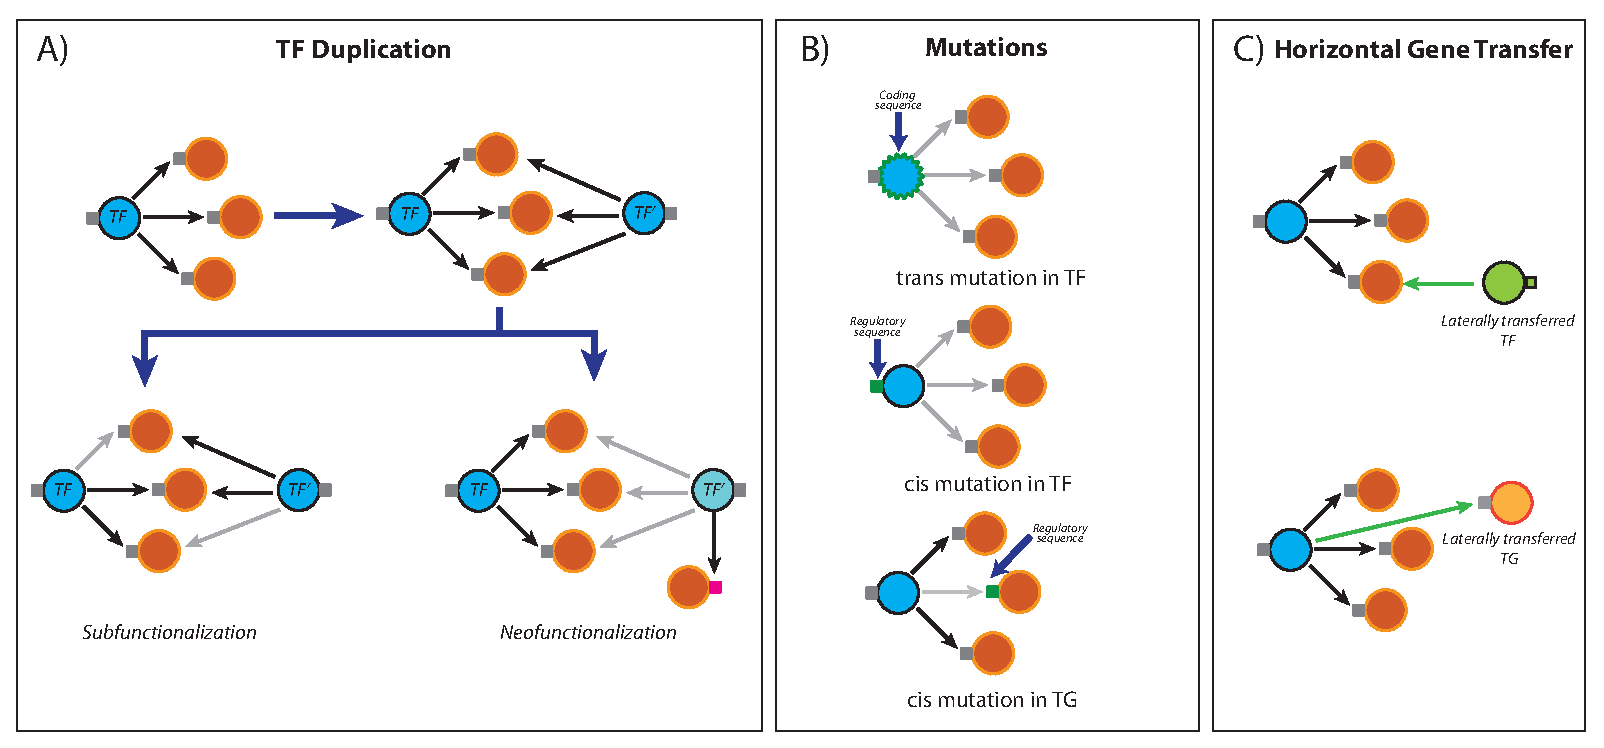
\includegraphics[width=0.7\textwidth]{figures/review_figure2}
 	\caption[Evolution of gene regulatory networks]{
 	Several molecular mechanisms mediate topological changes within GRNs. (A) Duplication of transcription factor (TF) and/or target genes (TG). Duplicated copies of a TF or downstream gene initially share the same interactions as its ancestor. Following duplication, however, either copy can subfunctionalize to contain a subset of those ancestral connections or neofunctionalize by gaining new interactions. Sub- and neofunctionalization generally occur via random mutations. (B) Mutations can occur in the coding or \textit{cis}-regulatory sequences of either TFs or TGs. Mutations in the cis-regulatory sequences of a TG only affect interaction with that particular target, while mutations in coding and cis regions of TF may affect all downstream interactions. (C) Microbial genomes can be extensively modified by horizontal gene transfers. Genomes can horizontally inherit new TF (green circle), TG (yellow circle) or both TF and its target simultaneously (not shown). Transcription factors and target genes are depicted in blue and orange circles respectively. \textit{Cis}-regulatory regions are denoted by gray boxes attached to the circles.
}
    \label{fig:chap4:evoGRN}
\end{figure}   

\section{Evolution of Gene Regulatory Networks (GRNs)}

If an organism is challenged by an environmental stress, individuals within the population harboring rewired GRNs that better negotiate the environmental change may enjoy a selective advantage. Here we describe common mechanisms by which GRNs become rewired during evolution, each of which is depicted in Figure \ref{fig:chap4:evoGRN}.   

\paragraph{Mutation}. Mutational events in transcription factors (TFs) can modify the specificity or affinity of TF DNA binding domains, such as mutations in the base contacting residues of DNA binding proteins that lead to recognition of multiple target DNA sequences \cite{luscombe_protein-dna_2002}, or affect protein-protein interaction domains that confer combinatorial specificity to gene regulatory programs \cite{baliga_is_2000}. In \textit{Halobacterium}, expansion of the general transcription factors allows for many possible TF-interactions \cite{feller_life_2007}, each of which may uniquely control cellular physiology \cite{facciotti_general_2007}. Rewiring may also occur by mutation in downstream target genes. In yeast, the rapid loss of \textit{cis}-regulatory motifs from multiple genes enables cells to grow rapidly under anaerobic conditions \cite{ihmels_rewiring_2005}.

\paragraph{Gene Duplication}. Duplication events are common in microbial genomes. Duplicated genes constitute a genetic toolbox that cells can harness to innovate and expand their phenotypic repertoire \cite{teichmann_gene_2004,gevers_gene_2004}.  Nearly half of the regulatory interactions in \textit{E. coli} and yeast appear to evolve through this process \cite{teichmann_gene_2004}.  Functional divergence of duplicated genes (neofunctionalization and subfunctionalization) can contribute to the development of new cellular functions  \cite{li_molecular_1997} or specialization in a condition-specific manner \cite{wapinski_gene_2010}. Whole genome duplications, though rare, can also contribute to evolution of GRNs \cite{kellis_methods_2004}. 

\paragraph{Horizontal gene transfer (HGT)}.  In prokaryotes, a large proportion of genes have been acquired laterally from different microbial species \cite{koonin_horizontal_2001} or even viruses \cite{rohwer_viruses_2009}. Eukaryotic-derived aminoacyl tRNA synthetases \cite{woese_aminoacyl-trna_2000}, antibiotic-resistance genes \cite{davies_origins_1996}, and numerous stress-response genes \cite{nelson_evidence_1999} are acquired in diverse lineages through HGT. While entire functional modules may be captured in this way, foreign DNA segments must often be integrated under the control framework of the new host, which can take tens of millions of years \cite{lercher_integration_2008}   







 

 
 